\section{Berenike Banek}

\subsection{Działanie}

\begin{displaymath} 
    \alpha = \sum_{k=1}^{n} \frac{1}{k} - \ln{n}
    \label{fig:equation}
\end{displaymath}

\subsection{Zdjecie}
\begin{figure} [h!]
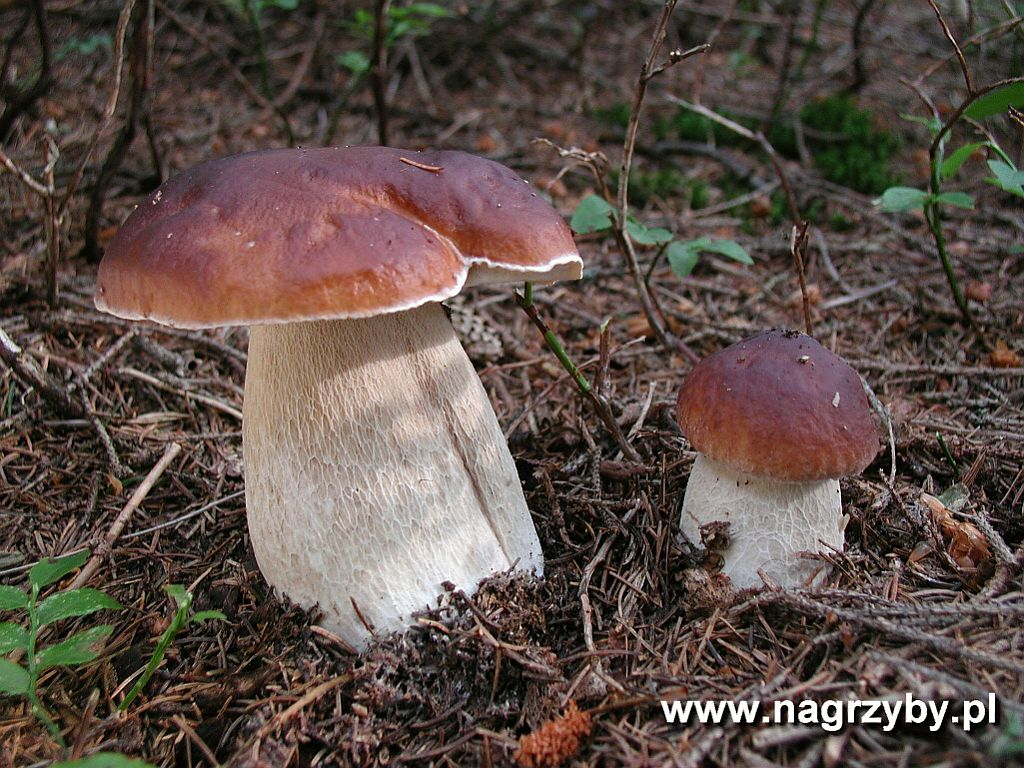
\includegraphics[width=0.6\textwidth]{pictures/grzyb.jpg}
\caption{Borowik}
\label{fig:mushroom}
\end{figure}

Tabela~\ref{fig:table6}
\subsection{Tabela}
\begin{figure} [h]
\begin{center}
\begin{tabular}{ |c|c|c| } 
 \hline
 \textbf{TABELA} & \textit{kolumna 1} & \textit{kolumna 2} \\ 
 \hline
 \underline{wiersz 1} & komórka 1 & komórka 2 \\ 
 \hline
 \underline{wiersz 2}  & komórka 3 & komórka 4 \\ 
 \hline
 \underline{wiersz 3}  & komórka 5 & komórka 6 \\ 
 \hline
\end{tabular}
\end{center}
\caption{Tabela 6}
\label{fig:table6}
\end{figure} 

\subsection{Lista nienumerowana:}
\begin{itemize}
  \item item 1
  \item item 2
  \item item 3
\end{itemize}

\subsection{Lista numerowana:}
\begin{enumerate}
  \item item 1
  \item item 2
  \item item 3
\end{enumerate}

\begin{flushleft}
\subsection{Krótki tekst}
\hspace{0.5 in} \textbf{Borowik szlachetny} (patrz: figure ~\ref{fig:mushroom}) – gatunek grzybów z rodziny 
\textit{borowikowatych}, potocznie nazywany prawdziwkiem.
W Polsce czesto spotykany zwlaszcza w gorach, rzadziej na nizu,
zwykle rzadki w \underline{okolicach wielkich miast.}\par
\hspace{0.5 in} 
\textbf{\textit{Aromatyczny}} grzyb jadalny o \textit{szerokich zastosowaniach}
w kuchniach \underline{europejskich.} 
Nadaje sie do bezposredniego spozycia, marynowania,
suszenia i do wszelkich innych rodzajów \textbf{przerobu}. 
Jest wykorzystywany w \textit{przemyśle spożywczym}.
\end{flushleft}